\secnumbersection{INTRODUCCIÓN}

\section{Contexto y motivación}
En la última década, la radioastronomía ha revelado la existencia de fenómenos transitorios extremadamente breves y energéticos, entre los que destacan las \textit{ráfagas rápidas de radio} (Fast Radio Bursts, FRBs). Las FRBs son pulsos de emisión de radio de duración del orden de milisegundos, generalmente originados a distancias extragalácticas. Su descubrimiento inicial en 2007 marcó un hito por la intensidad y lejanía de estas señales \cite{Lorimer2007}. El estudio de las FRBs es de gran relevancia científica: estas ráfagas pueden utilizarse como trazadores del medio intergaláctico, aportando información sobre la distribución de materia bariónica y sobre campos magnéticos a escalas cosmológicas, además de ofrecer nuevas oportunidades para la cosmología observacional \cite{Petroff_2022}. 

\begin{figure}[h]
\centering
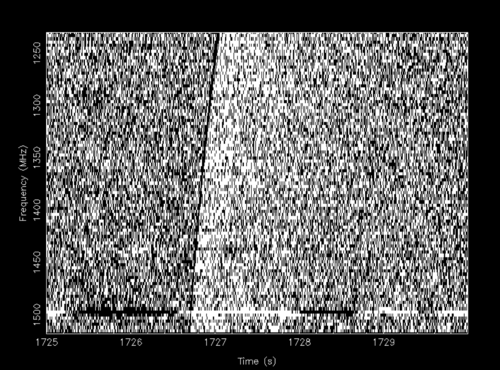
\includegraphics[width=0.8\textwidth]{figures/Lorimer Burst.png}
\caption{Ráfaga de Lorimer: observación de la primera ráfaga de radio rápida detectada, tal como la describió Lorimer en 2006.}
\label{fig:lorimer}
\end{figure}

\section{Problema}
Detectar FRBs en tiempo de procesamiento plantea desafíos considerables. Los radiotelescopios modernos generan volúmenes masivos de datos, lo que dificulta el procesamiento eficiente de observaciones en busca de eventos de milisegundos. A esto se suma la abundante interferencia de radiofrecuencia (RFI) de origen humano, que contamina las señales e imita pulsos astrofísicos, produciendo grandes listas de candidatos falsos. Los métodos tradicionales de búsqueda de pulsos individuales como los algoritmos implementados en suites clásicas tipo PRESTO y Heimdall se basan en dedispersión exhaustiva y umbrales fijos de detección, si bien han sido exitosos, son propensos a listas extensas de falsos positivos y requieren inspección manual intensiva, lo que limita su uso en operación en tiempo (casi) real \cite{CordesMcLaughlin2003, Ransom_2003, Barsdell_2012}. Por otra parte, \textbf{DRAFTS} aporta modelos de detección y clasificación, pero no un pipeline operativo extremo a extremo.

\textbf{TODO (Problema específico)}: Completar con 3–4 frases que describan el vacío exacto en tu contexto (datos disponibles, limitaciones de herramientas actuales en tu entorno, necesidad de near-real-time, etc.).

\section{Objetivos}
\textbf{Objetivo general:} Diseñar e implementar un pipeline basado en DRAFTS para detección y clasificación de transientes de radio, y extenderlo a regímenes de alta frecuencia.\\
\textbf{Objetivos específicos:}
\begin{itemize}
  \item Integrar y operacionalizar los modelos de DRAFTS en un pipeline reproducible.
  \item Diseñar módulos de ingesta, preprocesado, detección, clasificación y reporte.
  \item Adaptar la búsqueda a frecuencias milimétricas (mm-wave) considerando sus particularidades.
  \item Evaluar desempeño (recall, precision, F1, latencia) en banda L y en mm-wave.
\end{itemize}

\textbf{TODO (Medición de objetivos)}: Indicar cómo verificarás cada objetivo (p.ej., latencia \(<\) N s/archivo de 32 GB; F1 \(>\) X en FRB121102).

\section{Preguntas de investigación e hipótesis}
¿Cómo se comporta la detección y clasificación de FRBs al comparar banda L con mm-wave? Hipótesis: la atenuación del patrón bow-tie en mm-wave disminuye sensibilidad de detectores basados en tiempo–DM, mitigable ampliando rango/step de DM y mediante validación por sub-bandas y clasificación a DM\(\approx 0\).

\textbf{TODO (Criterios de falsación)}: Expresar qué resultados refutarían/confirmarían la hipótesis (p.ej., recall relativo mm-wave/L-band, tasa de falsos DM\(\approx\)0).

\section{Principales contribuciones técnicas}
\begin{itemize}
  \item Pipeline DRAFTS-MB con módulos definidos, contratos I/O y configuración.
  \item Estrategias de chunking/slices/overlap con criterios formales de \(\Delta DM\) por smearing.
  \item Integración CenterNet (detección) + ResNet (clasificación) con umbrales robustos (MAD/IQR).
  \item Extensión y validación en mm-wave y lineamientos para operación near-real-time.
\end{itemize}

\textbf{TODO (Evidencias de contribución)}: Enumerar outputs verificables (scripts, configs, artefactos, figuras clave, IDs de commit).

\section{Alcance y limitaciones}
El trabajo se enfoca en búsqueda de pulsos individuales (single-pulse) y no aborda timing ni localización interferométrica plena. Se trabaja con PSRFITS/FIL, con disponibilidad de GPU estándar. Limitaciones incluyen RFI a DM\(\approx 0\), dependencia de metadatos fiables y variabilidad instrumental.

\textbf{TODO (Límites explícitos)}: Añadir supuestos concretos (p.ej., resolución temporal mínima, anchos de banda soportados, formatos exactos, versiones de librerías).

\section{Organización del documento}
Este documento se organiza en diez capítulos más anexos. El Capítulo 2 presenta el marco teórico; el 3, el estado del arte; el 4, los requisitos y el diseño del pipeline; el 5, la implementación; el 6, la metodología experimental y los datasets; el 7, los resultados en banda L; el 8, la extensión a mm-wave (ALMA); el 9, la discusión y amenazas a la validez; y el 10, las conclusiones y trabajo futuro.

\section{Posicionamiento frente a pipelines en tiempo real}
Como motivación y punto de comparación, se discuten arquitecturas operativas de CHIME/FRB, ASKAP/CRAFT y MeerTRAP, destacando diferencias en adquisición, backend, mitigación de RFI y criterios de decisión, que orientan los requisitos y decisiones del presente pipeline.